\section{Limitations of NISQ hardware}
\label{sec:nisq}
Quantum hardware have been physically realised and even outperforms classical computers in very contrived situations \cite{arute2019, zhong2020, madsen2022}, but the hardware is still very limited.
The hardware is limited in the number of qubits, the connectivity between the qubits, and the noise and decoherence of the qubits.
It is believed that quantum hardware will continue to improve and eventually perform demanding algorithms like Shor's for large numbers.
Once enough qubits are available and error rates low enough, error correction schemes can be implemented, permitting fault-tolerant quantum computing and truly enable quantum supremacy.
Still, the era dubbed NISQ (Noisy Intermediate-Scale Quantum) is the first step, and to make use of the hardware, the inherent noise and its consequences must be understood, and algorithms must take the following limitations into consideration.

\subsection{Quantum channels and decoherent noise}
The unitary gates from \cref{sec:quantum_operations} are an idealisation, and in reality, the gates are not perfect.
A more realistic description of the gates is given by quantum channels, which can take noise into account.
In an unmeasured, ideal quantum system, the state evolution is veritably unitary, but as the system in practice does interact with the environment, this can be modelled as a quantum channel in which traditionally probabilistic noise is introduced.

Take the $X$-gate as an example.
If the fails to apply with probability $p$, the resulting density operator $\rho'$ can be expressed as
\begin{equation}
    \rho' = p\rho + (1-p)X\rho X^\dagger,
\end{equation}
where $\rho$ is the initial density.
Such a channel has eigenvalues $p$ and $1-2p$, where $I$ and $X$ share the former and $Y$and $Z$ the latter.
Consequently, states with $Y$- or $Z$-components will have mixing introduced.
Geometrically, this can be interpreted as contraction of states on the Bloch sphere towards the centre, illustrated in \cref{fig:noise_bloch}.

\begin{figure}
    \centering
    \begin{tikzpicture}
        \begin{groupplot}[
                group style={
                        group size=2 by 1,
                        horizontal sep=0pt,
                    },
                width=\textwidth,
                % height=30 cm,
                ymin = -1.5, ymax = 1.5,
                xmin = -1.5, xmax = 1.5,
                zmin = -1.5, zmax = 1.5,
                % grid=major,
                axis equal,
                axis lines = center,
                xlabel = {$x$},
                ylabel = {$y$},
                zlabel = {$z$},
                xtick = {-1, 0, 1},
                ytick = {-1, 0, 1},
                ztick = {-1, 0, 1},
                % enlargelimits=0.3,
                view/h=120,
                view/v=30,
                scale uniformly strategy=units only,
            ]
            \nextgroupplot
            \addplot3[
                opacity = 0.35,
                surf,
                fill=white, point meta=0,
                z buffer = sort,
                samples = 21,
                variable = \u,
                variable y = \v,
                domain = 0:180,
                y domain = 0:360,
            ]
            ({cos(u)*sin(v)}, {sin(u)*sin(v)}, {cos(v)});;
            \nextgroupplot[xshift=-3cm]
            \addplot3[
                opacity = 0.35,
                surf,
                fill=white, point meta=0,
                z buffer = sort,
                samples = 21,
                variable = \u,
                variable y = \v,
                domain = 0:180,
                y domain = 0:360,
            ]
            ({cos(u)*sin(v)}, {0.6*sin(u)*sin(v)}, {0.6*cos(v)});
        \end{groupplot}
        % add arrow from north on fig 1 to north on fig 2 
        \draw[->, shorten >=0.5cm,shorten <=1cm]
        ([yshift=-2.5cm] group c1r1.north)
        edge[bend left]
        node[midway,above] {\footnotesize Noisy $X$-gate}
        ([yshift=-2.5cm] group c2r1.north);
    \end{tikzpicture}
    \caption{
        Illustration of applying a noisy $X$-gate on the Bloch sphere.
        The left plot shows the set of all pure states, the Bloch sphere.
        On the right, the same set of states is shown after the application of a noisy $X$-gate with probability $p=0.2$ of failing.
        There, the $y$- and $z$-axes are contracted towards the centre by a factor $1-2p=0.6$, introducing mixing.
    }
    \label{fig:noise_bloch}
\end{figure}

Any physical gate will suffer some such noise, and so the tendency will be for states to degenerate towards the mixed centre of the Bloch sphere (or its higher-dimensional analogue).
Furthermore, measurements, letting a qubit idle when operating on others and even the preparation of the initial state $\ket{0}^{\otimes n}$ will suffer from decoherence.

This noise is very hard to avoid, as controlling the qubits necessarily requires some interaction with the environment.
Additionally, to operate on multiple qubits, a connection between them is required, which too will suffer from noise.
Nature tends to work against large quantum systems, made evident by the absence of quantum effects in regular life.

Due to the multiplicative effect of noise, the overall degeneracy will increase exponentially with the number of operations.
This means that there will be limits to the number of operations that can be performed before the system becomes unusable, assuming no error-correction is done.

\subsection{Coherent noise}
There may also be systematic errors in the unitary gates applied.
This kind of noise, known as coherent noise does not need quantum channels to be modelled, but may rather be modelled simply by slightly different unitary gates.
Here too, the $X$-gate can serve as an example.
Such a gate is typically implemented by applying a Hamiltonian for some time, requiring calibration of said time.
%
If it is not calibrated correctly, the effective operation will be a rotation that slightly deviates from the intended half turn.
When a gate like the $X$-gate is applied many times, even small errors will add up, which could cause an overall rotation of the state by a significant angle.

\begin{figure}
    \centering
    \begin{tikzpicture}
        \begin{axis}[
                width=0.6\textwidth,
                height=0.4\textwidth,
                xlabel = {Number of $X$-gates applied},
                ylabel = {Correct measurements (\%)},
                y filter/.code={\pgfmathparse{#1*100}\pgfmathresult},
                grid = major,
                % ytick = {0.1, 0.2, 0.3, 0.4, 0.5, 0.6, 0.7, 0.8, 0.9, 1},
            ]
            \addplot[
                color = blue,
                mark = none,
                % samples = 100,
                % domain = 0:100,
            ]
            table[x = n, y = p, col sep=comma] {../code/noise_fig/noise.csv};
            % add exponential dampening to the plot
            \addplot[
                color = gray,
                dashed,
                mark = none,
                samples = 100,
                domain = 0:1000,
            ]
            {0.5*(1+(1-2*0.003)^x)};
            \addplot[
                color = gray,
                dashed,
                mark = none,
                samples = 100,
                domain = 0:1000,
            ]
            {0.5*(1-(1-2*0.003)^x)};
            \addplot[
                color = gray,
                densely dotted,
                mark = none,
                samples = 100,
                domain = 0:1000,
            ]
            {0.5*(1 + cos(x))};
            \addplot[
                color = black,
                solid,
                mark = none,
                samples = 100,
                domain = 0:1000,
            ]
            {0.5*(1+cos(x)*(1-2*0.003)^x)};
        \end{axis}
    \end{tikzpicture}
    \caption{
        Proportion of correct measurements of a qubit after applying several noisy $X$-gates.
        The error in the rotation is \ang{1}, while the probability of failing to apply the gate is $p=0.3\%$.
        For each number of gates, the measurement is repeated 1000 times.
        The coherent error causes a sinusoidal behaviour, in which 180 rotations causes the overall rotation to be completely opposite.
        The decoherent error causes an exponential dampening, as the state becomes more and more mixed.
        The wiggly pattern stems from the shot noise, simply classical randomness stemming from the probabilistic measurement with a finite number of samples.
    }
    \label{fig:noise_graph}
\end{figure}

\Cref{fig:noise_graph} shows the effects of both coherent and decoherent noise on the measurement of a qubit after applying several noisy $X$-gates.
Clearly, information is quickly lost as the quantum state ends up different from what is expected and as the system becomes more and more mixed, losing quantum properties and instead obeying classical probabilities.
Even though current hardware suffers much less noise than the figure shows, NISQ algorithms must nonetheless be shallow, meaning that the amount of gates applied before measurement is small.
There are more sources of noise than the two included in the figure, and having to deal with multiple qubits certainly does not help.

\subsection{Qubit counts and connectivity}
\begin{figure}[b]
    \centering
    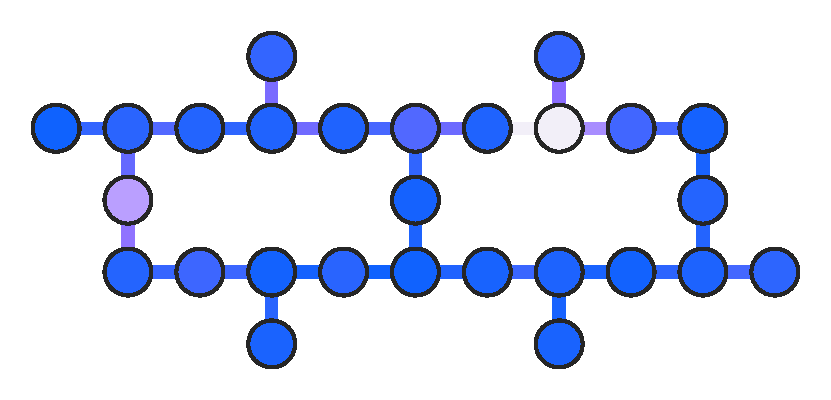
\includegraphics[width=0.65\textwidth]{connectivity.pdf}
    \caption{
        Qubit connectivity and error rates in IBM's 127-qubit Eagle r3 chip \cite{ibm_eagle}.
        Brighter coloured nodes indicate more $X$-errors, while brighter edges indicate more CNOT-errors.
        Only the CNOT-, $R_Z$-, $X$- and $\sqrt{X}$-gates are available.
    }
    \label{fig:connectivity}
\end{figure}
Another limiting factor is the amount of qubits.
Current hardware has around 10 to 100, which though still may be enough to express states too large for classical computers, is not enough to perform the most demanding algorithms.
Recent estimates find that millions of noisy qubits would be needed to break RSA encryption \cite{gidney2021}.

Another current limitation is the connectivity between the qubits.
Consider for example the connectivity graph in \cref{fig:connectivity}.
Qubits are generally only linked to two neighbouring qubits.
Moreover, only a basis set of gates will be directly available.
All this means that qubits may have to be swapped, often many times, and that multiple gates may be needed where only was intended.
This increases circuit depths, which in turn exacerbates the effects of noise.
